\subsection{C8 -- Saturn ring and moon shell witness}\label{app:c8}
\paragraph{Question.} Does the cited Saturn ring family, together with a selected moon witness set, provide a direct multi-shell orbital rendering showing ordered bands and satellite insertion on the same shell ledger?

\paragraph{Cited input block.} Familiar ring facts are taken from NASA's Saturn facts page and Cassini ring resources, including the overall extent of the main ring system and the named ring/gap structure.\footnote{NASA, \href{https://science.nasa.gov/saturn/facts/}{Saturn Facts}; NASA Cassini, \href{https://science.nasa.gov/mission/cassini/science/rings/}{Cassini: Saturn Rings}; NASA, \href{https://science.nasa.gov/resource/a-full-sweep-of-saturns-rings-with-labels/}{A Full Sweep of Saturn's Rings (with labels)}.} Semimajor axes and sidereal periods for selected Saturnian moons are taken from the JPL planetary-satellite mean-elements tables.\footnote{JPL Solar System Dynamics, \href{https://ssd.jpl.nasa.gov/sats/elem/}{Planetary Satellite Mean Elements}.}

\paragraph{Declared reduction.} Saturn is treated as a source ominion carrying the ordered shell family
\[
\Sigma_{\mathrm{sat}} = [\mathrm{saturn},[\mathrm{D},\mathrm{C},\mathrm{B},\mathrm{A},\mathrm{F},\mathrm{G},\mathrm{E}],[\mathrm{mimas},\mathrm{enceladus},\mathrm{tethys},\mathrm{dione},\mathrm{rhea},\mathrm{titan}]],
\]
with the ring bands retained as multiple shells and the selected moons retained as outer shell witnesses on the same cited ledger.

\paragraph{Readout.}
\begin{itemize}
\item cited system $\Sigma_{\mathrm{sat}}$
\item structural key \texttt{tetron:*:[saturn,rings]:6}
\item shell family read on the same ordered orbital ledger
\item rendered ring extent, Cassini Division, and selected moon orbits attached afterward
\end{itemize}

\paragraph{Operator chain.}
\[
\text{shell-band extractor}
\to
\text{cadence extractor}
\to
\text{ring-shell witness / moon-shell witness}.
\]

\paragraph{Rendered shell manifest.}
\begin{center}
\footnotesize
\begin{tabularx}{\linewidth}{@{}lcccX@{}}
\toprule
Band / moon & Radius witness & Period witness & Role & Note \\
\midrule
D--E ring family & ordered inner shell set & shell family & ring witness & multiple visible shell bands with Cassini Division gap \\
Mimas & $185{,}539$ km & $0.942$ d & outer shell witness & first selected moon shell beyond the main rings \\
Enceladus & $237{,}948$ km & $1.370$ d & outer shell witness & compact icy moon shell \\
Tethys & $294{,}619$ km & $1.888$ d & outer shell witness & mid-shell witness \\
Dione & $377{,}396$ km & $2.737$ d & outer shell witness & mid-outer shell witness \\
Rhea & $527{,}069$ km & $4.518$ d & outer shell witness & broad outer shell witness \\
Titan & $1{,}221{,}870$ km & $15.945$ d & slow outer shell & large far-shell witness \\
\bottomrule
\end{tabularx}
\end{center}

\paragraph{Output row.}
\begin{center}
\begin{tabularx}{\linewidth}{@{}lXcX@{}}
\toprule
Row & Structural key & Gap witness & Shell note \\
\midrule
C8.A & \texttt{tetron:*:[saturn,rings]:6} & Cassini Division & ring family with retained outer moon shells \\
\bottomrule
\end{tabularx}
\end{center}

\paragraph{SI rendering block.} Familiar renderings attached after the row include a ring-system radial extent of about $282{,}000$ km and a Cassini Division width of about $4{,}700$ km on the cited shell family, together with the selected moon semimajor-axis and period witnesses listed above. The rendered point is not a single ring label but the visibly ordered ring--moon shell family.\footnote{NASA, \href{https://science.nasa.gov/saturn/facts/}{Saturn Facts}.}

\paragraph{Figure witness.}
\begin{figure}[H]
\centering
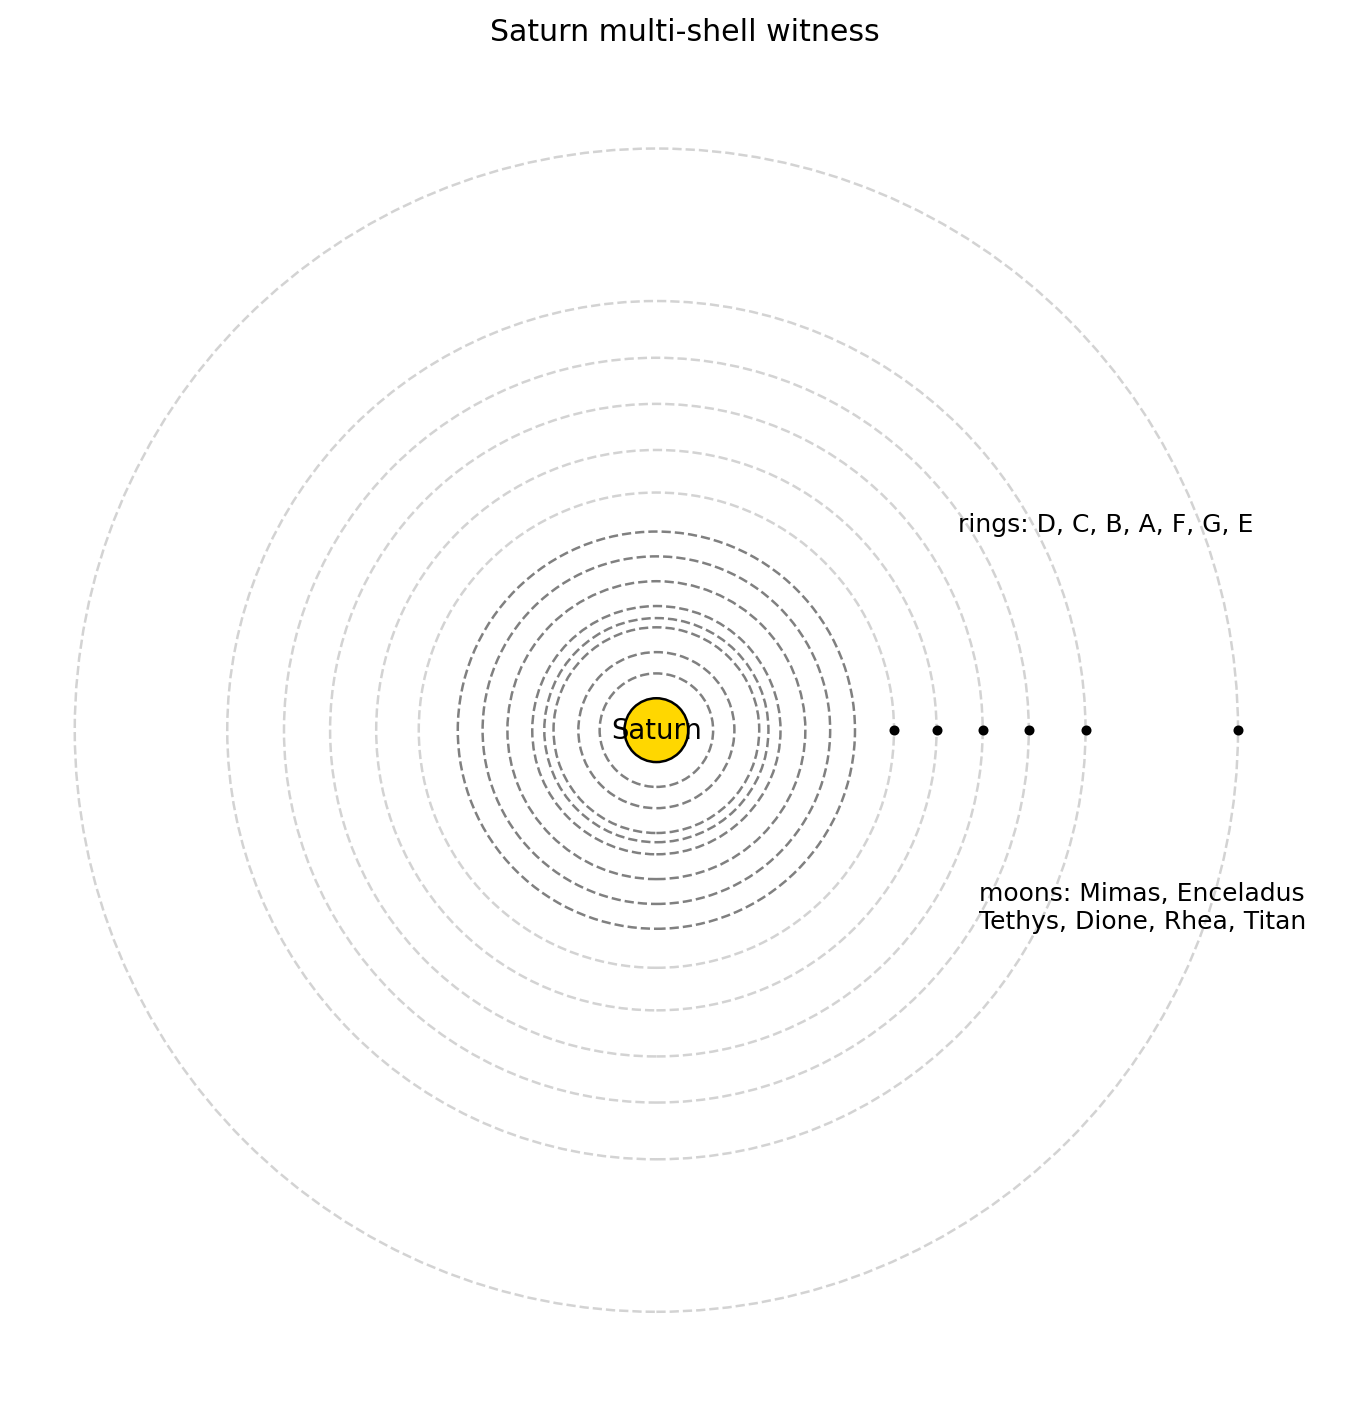
\includegraphics[width=0.74\linewidth]{figures/saturn/saturn_shell_family.png}
\caption{Saturn rings and selected moons as an explicit multi-shell witness. The rendered shell family is regenerated by the companion notebook and stored under the shared figures directory.}
\end{figure}

\FloatBarrier

\paragraph{Hook / Evidence.} Use the cited shell-band and cadence hooks. The point of this example is that Saturn's rings and selected moons display an immediately readable multi-shell family, making shell insertion explicit rather than implicit.

\paragraph{Companion notebook and manifest.} See Section~\ref{app:suppc-notebooks} for the executed calculation manifest and generated figure provenance for this section.

\begin{quote}\small\path{notebooks/saturn/c8_saturn_shells_worked.ipynb}\end{quote}
